\section{Discussion}

\subsection{Mortalité routière}

\subsubsection{Observation de carcasses}

Ces premiers résultats mettent en évidence la faible efficacité du drone et de la GoPro, comparativement à la méthode à pied, pour détecter les carcasses sur la chaussée (Fig.~\ref{fig:bar_mix_25}). La méthode par drone avait d'ailleurs été retirée du protocole pour l'échantillonnage de 2026, faute de détection en 2025. Les résultats issus des GoPro sont toutefois à nuancer. En effet, bien que peu performante par rapport à la méthode à pied, cette méthode a tout de même permis de détecter des carcasses de mammifères. Sur les six carcasses observées, une était une marmotte, deux des moufettes, deux des ratons laveurs et une dernière un mammifère indéterminé. En revanche, les enregistrements n'ont permis de détecter aucun anoure, oiseau ou reptile. Ainsi, dans le cadre de cette étude, seule la méthode à pied a permis de détecter l'ensemble des groupes de vertébrés, la GoPro se limitant aux vertébrés de taille moyenne.

Le protocole initial prévoyait d'associer aux inventaires par enregistrement GoPro des inventaires réalisés par observation directe depuis le véhicule. Cette combinaison devait permettre de quantifier la perte d'information entre le visionnement différé des enregistrements et le dénombrement des carcasses en temps réel. Les auxiliaires de recherche n'ont toutefois pas été en mesure d'appliquer conjointement les deux protocoles, de sorte que cette information ne pourra être obtenue dans le cadre des tronçons suivis actuellement. 

Des données quantitatives sur cette perte d'information devraient néanmoins être disponibles prochainement, puisque dans le cadre d'une collaboration avec un projet de suivi de la mortalité routière amorcé au printemps 2026 sur un tronçon de 14 km de l'autoroute 35, entre Saint-Sébastien et Saint-Armand. Ce projet vise notamment à quantifier la mortalité routière de l'herpétofaune dans ce secteur. Depuis le 19 mai 2026, deux auxiliaires de recherche y inventorient et dénombrent les carcasses présentes sur la chaussée selon trois méthodes. La première consiste à parcourir à pied les abords de la chaussée sur une section de 4,5 km, et ce, dans chaque sens de circulation. La deuxième couvre l'ensemble du tronçon de 14 km en véhicule. La troisième repose sur l'analyse différée des enregistrements d'une caméra GoPro fixée au véhicule durant l'inventaire en véhicule, ce qui permet de comparer directement les deux dernières méthodes. Au total, 206 visites ont été réalisées.

Bien que le visionnement des enregistrements GoPro reste à faire, il est déjà possible d'établir un premier comparatif entre les observations obtenues à pied et celles obtenues lors des parcours en véhicule sur le tronçon de l'A35 (Fig.~\ref{fig:bar_hor_bino26}). Ce portrait fait ressortir un profil semblable à celui observé lors de la phase II du projet R875. Les inventaires en véhicule ont ainsi permis de détecter très peu d'amphibiens, de reptiles et d'oiseaux, mais ont mené au dénombrement de 267 carcasses de mammifères. Comme dans le cas du projet R875, la majorité des mammifères détectés appartenaient à des espèces de taille moyenne, notamment le raton laveur (\textit{Procyon lotor}), l'opossum d'Amérique (\textit{Didelphis virginiana}) et la moufette rayée (\textit{Mephitis mephitis}).

Il importe toutefois de souligner que les inventaires en véhicule sur l'A35 ont été réalisés sur une distance de 14 km, soit une longueur nettement supérieure à celle des tronçons de 1 km utilisés dans le projet R875.1. Le tronçon de l'A35 était également visité à 52 reprises, un effort incomparable à celui effectué sur les tronçons du R875.1. Il est donc normal d'avoir des effectifs nettement supérieurs sur l'A35. De plus, les inventaires à pied sur l'A35 ont été effectués sur une section plus courte, afin d'être réalisables pour une petite équipe. Même si les conditions ne sont pas optimales pour comparer formellement les deux méthodes. Bien que ces conditions ne permettent pas une comparaison formelle des deux méthodes, elles suffisent à faire ressortir les grandes tendances qui se dégagent des observations obtenues par chacune d'elles.

\begin{figure}[H]
\centering
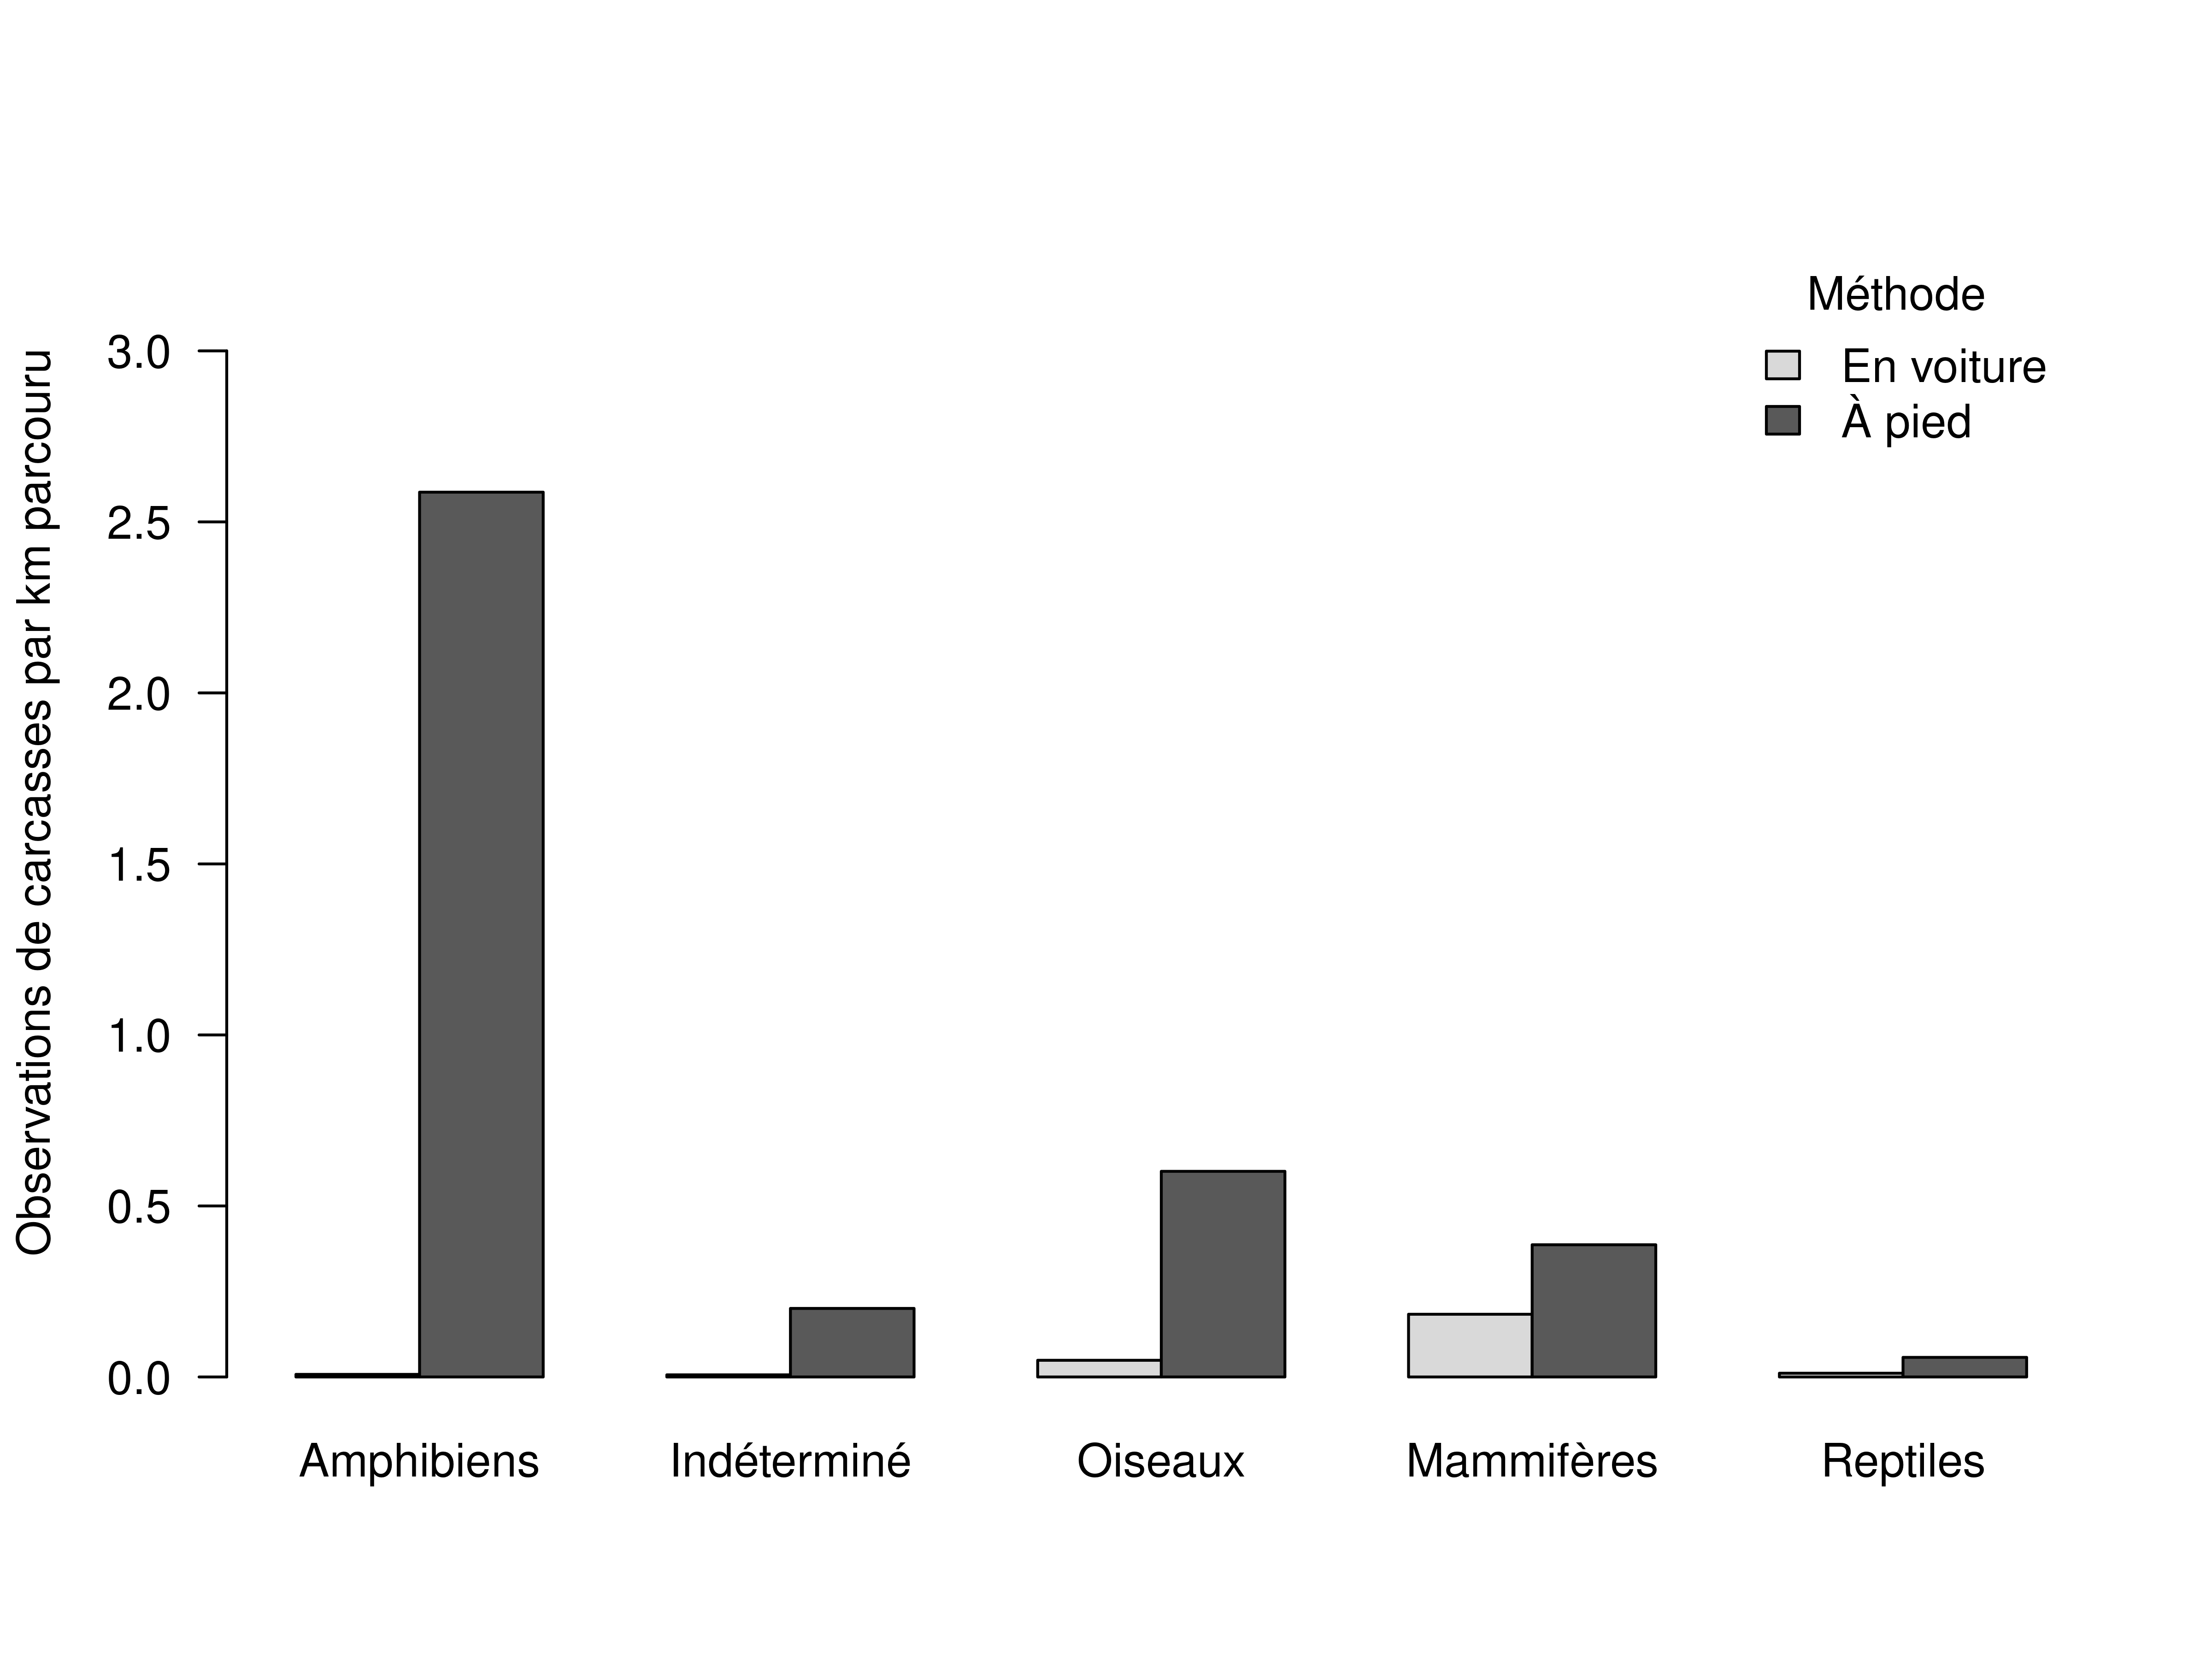
\includegraphics[width=0.8\textwidth]{figs_monteregie_liv3/morts_pond_2026.png}
\caption{Nombre de carcasses observées ramenées au kilomètre parcouru selon la méthode d'échantillonnage, sur un tronçon de l'A35. Données récoltées lors de 206 inventaires (104 en voiture, 102 à pied) réalisés du 19 mai au 21 août 2026. Les parcours en voiture englobent le tronçon inventorié à pied, mais s'étendent en amont et en aval sur un linéaire plus long avec potentiellement des habitats différents. De ce fait, ces écarts entre les deux méthodes traduisent  à la fois une différence de détectabilité inhérente à la méthode ainsi qu'une différence dans les habitats échantillonnés.}
\label{fig:bar_hor_bino26}
\end{figure}


\subsubsection{Persistance}

Globalement, les tests de persistances révèlent que peu de morceaux de poulet étaient prélevés par des prédateurs , soit seulement 12,3~\%. Dans le livrable précédent il avait déjà été constaté que la persistance apparaissait comme nettement plus faible sur d'autres projet actuellement en cours au Bas-Saint-Laurent ou au Nouveau-Brunswick. Par ailleurs le temps moyen de prédation était également assez long, soit environ 16 h 00.

\subsubsection{Enregistrements acoustiques et suivi des milieux humides}

Pour lLe modèle entraîné pour la grenouille du Nord et la grenouille léopard n'a détecté aucune grenouille du Nord parmi les 12 904 fichiers d'enregistrement de 2025. Il est peu probable que cette absence de détection soit attribuable à une faiblesse du modèle. En effet, les tests réalisés en laboratoire montrent que, malgré un taux élevé de faux positifs, le modèle détecte bien l'espèce lorsqu'elle est présente, et ce, même dans des contextes variés. Par ailleurs, l'absence d'observation de grenouille du Nord lors des inventaires visuels plaide pour une absence de l'espèce sur les sites. En revanche, ce qui paraît davantage surprenant c'est la faible occurence de la grenouille léopard sur l'ensemble des sites suivis. D'autres analyses avec l'outil birdNET seront faites pour le prochain livrable avec un nouveau modèle, entraîtné avec davantage de fichiers, ce qui permettra de valider définitivement ces premiers résultats. 

Initialement, le protocole des inventaires visuels prévoyait le dénombrement des adultes, des juvéniles, des larves et des masses d'\oe{}ufs. En 2025, les décomptes précis de masses d'\oe{}ufs par espèce n'ont pas pu être réalisés, l'identification et le dénombrement des pontes s'étant révélés trop exigeants pour être appliqués de manière fiable sur le terrain, seule la présence ou l'absence de masses d'\oe{}ufs a pu être consignée par les auxiliaires.

La rainette versicolore, espèce la plus fréquemment détectée par l'enregistrement acoustique passif, est celle dont le nombre d'occurrences était le plus faible lors des inventaires visuels. Ce contraste illustre la complémentarité des deux approches. En effet, les espèces de petite taille et avec des m\oe{}urs arboricoles, telles que la rainette versicolore, sont difficiles à localiser dans la végétation. Il est donc attendu que cette espèce soit mieux détectée par les méthodes passives que par la recherche active.

À l'inverse, des espèces de plus grande taille et se trouvant facilement en bordure des étangs se prête mieux à des inventaires visuels. Néanmoins, il est tout de même surprenant que la grenouille verte ne soit pas davantage détectée par l'intermédiaire du dispositif d'enregistrement passif. Il est possible que l'emplacement utilisé pour positionner l'audiomohts ne soit pas optimal pour détecter les espèces sur un endroit. 

Le fait que la grenouille des bois n'ait pas été détecté est potentiellement dû à un début d'échantillonnage trop tardif. 

